% ============================================== %
% PROPOSED METHODS %
% ============================================== %

%\vspace{-7pt}

\section{The D\texorpdfstring{\MakeLowercase{i}}{}VE Schemes with Pruning}\label{sec:pruning}
%\risch{
%\mas{
As described above, both DiVE-Greedy and DiVE-Swap execute all the underlying queries for each view $X_i$ in $X$. 
%
However, only a small fraction of those views is actually included in the final top-k recommended set. 
%
Consequently, a significant amount of query processing cost is incurred for generating low-utility views. 
%
Thus, in this section, we propose efficient techniques for pruning such low-utility views without incurring the high cost for evaluating their importance score (Sec. ~\ref{subsec:pruning-Swap} and Sec. ~\ref{subsec:pruning-Greedy}).
Moreover, we also propose an adaptive pruning method based on {\em non-parametric predictive intervals} (Sec. ~\ref{subsec:adaptive-pruning}). 
%
Such method is able to balance the tradeoff between minimizing the number of executed queries and maximizing the quality of recommendation. 

% 
%}

\eat{
Thus, we propose some pruning techniques in Sec. ~\ref{subsec:pruning-Greedy-Swap}, that leverage the diversity score to bound the maximum utility score achieved by each view $X_i$, and in turn allows for pruning low-utility views without incurring the high cost for evaluating their importance.
In addition, we also propose adaptive pruning method in Sec. ~\ref{subsec:adaptive-pruning}, which based on {\em non-parametric predictive intervals}. This adaptive pruning method is able to balance the tradeoff between minimizing the number of executed queries and maximizing the effectiveness. 
}


\subsection{Pruning for DiVE-Swap}
\label{subsec:pruning-Swap}

In Sec. ~\ref{subsec:dive-swap}, we presented two variants of DiVE-Swap: 1) \textit{DiVE-iSwap}, and 2) \textit{DiVE-dSwap}.
%
While those two variants incur the same cost, they offer substantially different performance when combined with our pruning techniques. 
%
Particularly, consider DiVE-iSwap, which is initialized with the $k$ views that maximize importance. 
%
%\risch{
%	To select those views, all possible views have to be generated first, which in turn requires processing all their corresponding queries such as on {\em Linear-Importance}. 
%	%
%	The difference between DiVE-iSwap and Linear-Importance is the objective function itself, while Linear-Importance only consider importance score whereas DiVE-iSwap uses hybrid objective function (i.e., Eq.\ref{objectif_function}).
%}
%
To select those views, all possible views have to be generated first, which in turn requires processing all their corresponding queries. 
%
Hence, DiVE-iSwap simply eliminates all opportunities for pruning as all views are executed in the initialization phase. 
%
To the contrary, DiVE-dSwap is initialized with the $k$ views that maximize diversity.
%
To select that initial set, no query execution is needed and the processing is limited to computing the context-based deviation distances, which incurs  a significantly lower processing cost compared to query execution. 
%
Hence, DiVE-dSwap provides a valuable opportunity for pruning low-utility views. 


Recall that under DiVE-dSwap, in each iteration a view $X_i \in X$ is selected to replace a view $S_j \in S$. 
%
The criterion for that selected view is to improve $F\left(S\right)$. 
%
That is, $F(S \backslash S_j \cup X_i) >  F(S)$. 
%
Hence, the task is to find that {\em top-1} pair of views $<X_i, S_j>$ that provides the maximum improvement in $F\left(S\right)$ once interchanged. 
%
Without pruning, that requires iterating through $S$ and $X$ simultaneously and computing $F$ for each pair, which requires processing and generating each view in $X$. 
%
To avoid such expensive processing and enable pruning, the following steps are taken. 
%

A list $L$ is created for all possible swap pairs $<X_i, S_j>$, where $L$ is sorted based on the diversity achieved if the swap is to be made. 
%
%
Notice that up to this point the only processing needed is to compute diversity without any query execution to evaluate the importance of any $X_i$. 
%
%
Given that setting, the task is clearly similar to top-k query processing, for which numerous optimization tehniques are proposed (e.g.,\cite{Fagin:2003:CTK:644108.644113, Ilyas:2008:STK:1391729.1391730}).
%
Particularly, to find the {\em top-1} view, each view $X_i$ is initially assigned an importance equal to the upper bound $I_u$(Sec. ~\ref{subsec:problem_definition}). 
%
In turn, the upper bound of $F\left(S\right)$ achieved by $X_i$ is computed as: $maxF(S \backslash S_j \cup X_i)$, which is based on the actual diversity achieved by the swap, and the upper bound on importance.
%
As such, $maxF(S \backslash S_j \cup X_i)$ is compared against $F(S)$, leading to one of the following two cases:
%
If $maxF(S \backslash S_j \cup X_i)$ > $F(S)$, then the swap $<X_i, S_j>$ can ``potentially'' improve $F\left(S\right)$. 
%
Hence, at that stage the view $X_i$ needs to be generated in order to evaluate its actual importance $I(X_i)$. 
%
Otherwise, the pair $<X_i, S_j>$ is pruned if: 
\begin{center}
$maxF(S \backslash S_j \cup X_i) < F(S)$.
\end{center}


Simply put, if the upper bound  $maxF$ achieved by that swap is still less than the current $F(S)$, then the actual $F(S \backslash S_j \cup X_i)$ is guaranteed to be less than $F(S)$ and the pair $<X_i, S_j>$ can be safely ignored. 
%
More importantly, since the $L$ is sorted by diversity, then the next views are also guaranteed to provide no improvement and that iteration of DiVE-dSwap reaches {\em early termination}.  
%
Hence, for all the remaining views no query processing is needed, which significantly reduces the overall cost. 



	%It also can be implemented on Greedy %
%\subsubsection{ DiVE-Greedy Pruning} 
\subsection{Pruning for DiVE-Greedy}
\label{subsec:pruning-Greedy}

%\mas{
The pruning technique described above is directly applicable to DiVE-Greedy.
%
Particularly, recall that under DiVE-Greedy, in each iteration the view with the highest utility score is added to the partial set $S$ until $|S| =k$. 
% 
As described in Eq. ~\ref{utility_each_candidate}, such utility score $U(X_i)$ is a weighted sum of two measures: 1) the importance score of $X_i$ (i.e., $I(X_i)$), and 2) the distance of $X_i$ from $S$ (i.e., $ setDist\left(X_i, S\right)$).
%	
Thus, while the goal in DiVE-dSwap is to find the pair $<X_i, S_j>$ that provides the maximum improvement in $F\left(S\right)$, the goal for DiVE-Greedy is to find the view with the highest utility $U(H)$.  
%
Hence, similar to DiVE-dSwap, a list $L$ of all views in $X$ is created such that each $X_i$ is assigned an importance equal to the upper bound $I_u$ and $L$ is sorted based on the diversity score of each view $X_i$ to the current set $S$.
%
Then, the highest utility $U(H)$ is initialized to a default value of 0.0, and the list $L$ is traversed in order. 
%
For each visited view $X_i$, the upper bound on the utility achieved by $X_i$ (i.e., $maxU(X_i)$) is computed using its actual diversity score and the upper bound on its importance.
%
If $maxU(X_i) > U(H)$, then $X_i$ is generated and its actual utility $U(X_i)$ is calculated. 
%
Accordingly, if $U(X_i) > U(H)$, then $U(H)$ is set to be equal to $U(X_i)$. 
%
However, if $maxU(X_i) < U(H)$, then early termination is reached. 
%}



\eat{
	The pruning technique employed for DiVE-dSwap is directly applicable to DiVE-Greedy.
	%
	In DiVE-Greedy, in each iteration a view $X_i$ is selected to be added to set $S$ until $|S| =k$. % (Algorithm ~\ref{DiVE-Greedy} line 6).
	% 
	The criterion for that selected view is a view with highest utility score $U(X_i)$ (Algorithm ~\ref{DiVE-Greedy} line 5). 
	%
	That is, the utility score of each view $U(X_i)$ is a weighted sum of two measures: 1) the importance score of view $I(X_i)$ and 2) distance of a view from S $ setDist\left(X_i, S\right) $ (Eq. ~\ref{utility_each_candidate}).
	%
	The task is to find that {\em top-1} view that provide maximum improvement in $F(S)$. 
	%
	In order to employing our pruning technique to DiVE-Greedy, the following steps are taken.
	
	Similary to DiVE-dSwap, a list $L$ of all views in $X$ is created which is sorted based on the diversity score of each view $X_i$ to set $S$.
	%
	%The \textit{top-1} view in $L$ need to be executed to generate the current $F(S)$.
	%
	To find the \textit{top-1} view, $X_i$ is assigned an importance equal to the upper bound $I_u$. In turn, the $maxU(X_i)$ is computed using the actual diversity score and the upper bound on importance. 
	%
	Then, the query of {\em top-1} view is executed to get its importance score.
	%
	Since the actual importance score of {\em top-1} view has been known, the actual utility of {\em top-1} view $U$({\em top-1}) can be calculated. 
	%
	That is, if $maxU(X_i) < U$({\em top-1}) then $X_i$ is pruned and query for $X_i$ is not executed because there exists a {\em top-1} view which is guaranteed to provide higher utility value than $X_i$.
}

\subsubsection{DiVE-dSwap vs. DiVE-Greedy} 



At this point, it is especially important to examine and contrast the pruning power achieved by each of DiVE-Greedy and DiVE-dSwap. 
%
For DiVE-Greedy, recall that pruning is attained for those views where: $maxU(X_i) < U(H)$. 
%
However, since DiVE-Greedy is a constructive algorithm, the set $S$ is incrementally constructed iteration by iteration until $|S|=k$. 
%
Hence, in the first iterations $S$ has a very small number of selected views with a minimum of $|S|=2$. 
%
Naturally, when $S$ is a small set, then most of the remaining unselected views in $X$ are expected to exhibit high diversity, since the majority of them will be very dissimilar from the small set of views in $S$.
%
Accordingly, for most of the views in $X$, the value $maxU(X_i) $ will be relatively high, due to achieving high score on diversity. 
%
Hence, most views will fail to satisfy the pruning condition and are consequently executed incurring high query processing cost. 

To the contrary, DiVE-dSwap is initiated with a set $S$ of $k$ diverse views. 
%
Hence, it will initially have a reasonably high $F(S)$. 
%
Moreover, many views in $X$ will be ``close'' to some view in $S$. 
% 
Hence, the swaps that involve those views will score low on diversity, and in turn low $maxF$.
%
Since pruning happens when $maxF(S \backslash S_j \cup X_i) < F(S)$, the combination of those two factors above (i.e., high $F$ and low $maxF$) allows for many views satisfying the pruning condition, which improves the pruning power of DiVE-dSwap. 
%
That pruning power can be further improved by relaxing the assumption about maximum importance $I_u$, as described next.




\subsection{Predictive Interval for Adaptive Bounds}
\label{subsec:adaptive-pruning}
%Premble


%% I_u and its drawbacks
In general, both the pruning schemes provided by DiVE-Greedy and DiVE-dSwap rely on the fundamental idea of evaluating the upper bound of the benefit provided by a view $V_i$ towards the objective $F$. 
%
If that maximum benefit is still not enough to consider $V_i$ to join $S$, then $V_i$ is pruned and its query processing cost is saved. 
%
Moreover, to evaluate that upper bound, both schemes compute the actual diversity offered by $V_i$ and instead of computing its actual importance, it is substituted with the maximum attainable importance score $I_u$. 
%
Naturally, overestimating  $I(V_i)$ leads to overestimating its benefit and consequently limited pruning power is achieved. 
%
Meanwhile, for most datasets, $I_u$ is in fact an overestimation of $I(V_i)$. 
%
Hence, our goal in this section to provide a tighter bound on $I(V_i)$, which allows for maximum pruning while maintaining the quality of the solution. 
 

Recall that $I_u$ is achieved when for each group $a_i$, the corresponding value $\frac{g_i}{G}$ in $P[V_{i}(D_R)]$ or $P[V_{i}(D_Q)]$ is zero. 
%
Hence, $I_u$ is a theoretical bound for the maximum importance achieved by any view in any dataset.
%
For most real datasets, however, that condition is rarely satisfied and the actual upper bound $I_{au}$ is typically much smaller than $I_u$. 
%
Meanwhile, a hypothetical pruning scheme that utilizes that actual upper bound $I_{au}$ is expected to deliver more pruning power than the schemes using the theoretical upper bound $I_u$, especially when $I_{au}  \ll I_u$.
%
In practice, however, that hypothetical scheme is not achievable since obtaining the value $I_{au}$ requires executing all the possible views, which is clearly in conflict with the goal of pruning.

Accordingly, rather than using overestimated $I_u$ or obtaining the actual $I_{au}$, our goal is to estimate $I_{au}$ with high accuracy and minimum number of query executions. 
%
In particular, given the set of possible views $\mathbb{V}$, the goal is to estimate the maximum importance $\bar{I}_{au}$ given by some view in $\mathbb{V}$. 
%
However, estimating the maximum value of a population is known to be a challenging problem, as opposed to estimating other statistics such as average or sum \cite{Hu:2009:EAT:1516360.1516487}.
%
That challenge is further emphasized when the values exhibited by the population are skewed and do not follow a typical normal distribution, which is typically the case for the importance value of views.
 %
 
Thus, instead of estimating $I_{au}$, we rely on {\em non-parametric predictive interval} models to determine its value with certain level of confidence without any assumption on the population \cite{Hu:2009:EAT:1516360.1516487}. 
%
To apply that model, some sample views are executed and the maximum importance observed in that sample is recorded as $\bar{I}_{au}$. 
%
To determine the number of samples, a {\em Predictive Interval (PI)} is to be defined, such that: 	
$PI= \dfrac{\left(m-1\right) }{\left(m + 1\right)}$, where $m$ is the number of samples. 
%

For instance, setting $m = 19$, results in PI = 90\%. 
%
That is, 90\% of the time, the importance value of an unseen view $V_i$ will be less than the maximum importance seen so far. 
%
Clearly, the higher the PI value, the higher the accuracy of $\bar{I}_{au}$, but also requires executing more views.  
%
In this work, we find that a value of $PI=97\%$ is able to strike a fine balance between minimizing the number of executed queries and maximizing the objective $F$, as shown next.










\eat{
	\noindent{\bf DiVE-dSwap vs. DiVE-Greedy:} At this point, it is especially important to examine the pruning power achieved by each of DiVE-Greedy and DiVE-dSwap. 
	%
	For DiVE-Greedy, recall that pruning is attained for those views where: $maxF(S \cup X_i) < F(S)$. 
	%
	However, since DiVE-Greedy is a constructive algorithm, the set $S$ is incrementally constructed iteration by iteration until $|S|=k$. 
	%
	Hence, in the first iterations $S$ has a very small number of selected views with a minimum of $|S|=2$. 
	%
	Meanwhile, our context-driven consists of three components (i.e., attribute, measure, and aggregate function) as explained in Sec ~\ref{context-driven-deviation}.
	%
	Naturally, when $S$ is a small set and each view consists of three components ($A,M, F$) then many of the remaining unselected views in $L$ are expected to have same score of $ setDist(X_i, S) $.
	%
	Hence, this condition can decreases the chance of pruning due to many views are not satisfying the pruning condition. 
	
	To the contrary, DiVE-dSwap is initiated with a set $S$ of $k$ diverse views. 
	%
	Hence, the probability of views in $L$ to have same score of $setDist(X_i, S)$ not as high as DiVE-Greedy. 
	%
	This condition should improve the pruning power of DiVE-dSwap.
	% 
	Moreover, the pruning power can be further improved by relaxing the assumption about maximum importance $I_u$, as described next.
}

\eat{\noindent{\bf DiVE-dSwap vs. DiVE-Greedy:} At this point, it is especially important to examine the pruning power achieved by each of DiVE-Greedy and DiVE-dSwap. 
	%
	For DiVE-Greedy, recall that pruning is attained for those views where: $maxF(S \cup X_i) < F(S)$. 
	%
	However, since DiVE-Greedy is a constructive algorithm, the set $S$ is incrementally constructed iteration by iteration until $|S|=k$. 
	%
	Hence, in the first iterations $S$ has a very small number of selected views with a minimum of $|S|=2$. 
	%
	Naturally, when $S$ is a small set, then most of the remaining unselected views in $X$ are expected to exhibit high diversity, since the majority of them will be very dissimilar from the small set of views in $S$.
	%
	Accordingly, for most of the views in $X$, the value $maxU(V_i)$ will be relatively high, due to achieving high score on diversity especially in the first iteration of Greedy. 
	%
	%Hence, most views will fail to satisfy the pruning condition and are consequently executed incurring high query processing cost. 
	
	To the contrary, DiVE-dSwap is initiated with a set $S$ of $k$ diverse views. 
	%
	Hence, it will initially have a reasonably high $F(S)$. 
	%
	Moreover, many views in $X$ will be ``close'' to some view in $S$. 
	% 
	Hence, the swaps that involve those views will score low on diversity, and in turn low $maxF$.
	%
	Since pruning happens when $maxF(S \backslash S_j \cup X_i) < F(S)$, the combination of those two factors above (i.e., high $F$ and low $maxF$) allows for many views satisfying the pruning condition, which improves the pruning power of DiVE-dSwap. 
	%
	That pruning power can be further improved by relaxing the assumption about maximum importance $I_u$, as described next.
}


\eat{
	\mas{
		%Brief explanation for both techniques in terms of pruning%
		\sout{In the section before, there are two schemes: DiVE-Greedy and DiVE-Swap are proposed. 
			%
			DiVE-Greedy is a constructive type algorithm, which iteratively selects new views in $X$ to be added to set $S$. 
			%
			Meanwhile, DiVE-Swap is interchanging type algorithm, which interchanging views in $X$ to all views in set $S$ until no more views can be swapped between $X$ and $S$.   
			%
			Both schemes have substantially different techniques in term of generating the result set that has optimal $F(S)$, however, same pruning technique is applicable to be implemented to them. }
		
		\sout{In this section, due to the pruning technique is implemented in the same way to the both schemes, we want to focus the discussion to the one of schemes which is DiVE-Swap. }
		
		% 
		
		
		%Discussion Pruning on dSwap %
		
	}
	
}

%
%
%
%\eat{%HAK version
%	As mentioned in the previous section, the cost of the DiVE-Greedy algorithm is dominated by the cost of executing view queries and is proportional to the number of possible views. 
%	%
%	Although hundreds of views are possible for a given subset of data, only a small fraction of the views are actually of interest and are included in the top-k set. Consequently, a significant fraction of the query processing cost is incurred on evaluating low-utility views. Hence, in this section we propose a pruning technique to reduce the search space of views. 
%}
%
%
%
%
%\eat{
%	As mentioned in the previous section, the cost of the DiVE-Greedy algorithm is dominated by the query processing cost $C_Q$ and is proportional to the number of possible views. 
%	%
%	Although hundreds of views are generated for a given subset of data $D_Q$, only a small fraction of those views are actually of interest and are candidates to be included in the top-k set. 
%	%
%	As such, a significant fraction of the query processing cost is incurred in evaluating low-utility views. 
%	%
%	This  motivated us to propose a pruning technique to minimize the search space of views and narrow it down to the most promising ones, as follows. 
%	
%	DiVE-Greedy is an constructive type algorithm, it iteratively selects a new view to be added to set $S$. Particulary, in each iteration a view $X_i \in X$ is selected to be added to $S$. 
%	%
%	The criterion for that selected view is to improve $F\left(S\right)$. 
%	%
%	Hence, the task is to find {\em top-1} of $X_i$ that provide the maximum improvement in $F\left(S\right)$ once added to set $S$. 
%	
%	%
%	Without pruning, that requires iterating through $X$ simultaneously and computing $F$ for each $X_i$, which requires processing and generating each view in $X$. 
%	%
%	In order to avoid such expensive processing, the pruning technique is proposed as elaborated next. 
%	%
%	
%	A list $L$ is created for all candidate views in $X$, where $L$ is sorted based on the diversity (i.e., $setDist$) achieved if $X_i$ is to be added to set $S$. 
%	%
%	%
%	Until this step, there is no query executions needed, the cost only diversity cost to compute $setDist$ score of $X_i$ to set $S$. 
%	%
%	%
%	We propose {\em top-1} strategy that is similar to top-k query processing (e.g., \cite{Fagin:2003:CTK:644108.644113, Ilyas:2008:STK:1391729.1391730}).
%	%
%	Particularly, to find the {\em top-1} view, each view $X_i$ is initially assigned an importance equal to the upper bound $I_u$. 
%	%
%	
%	For instance, given list $L$ which sorted based on $setDist$ score. 
%	%
%	The query of first view $X_1$ in $L$ is executed, since the actual importance score of $X_1$ is known, the actual $F(S \cup X_1)$ can be calculated. 
%	%
%	Hence, this $F(S \cup X_1)$ will be the current $F(S)$. 
%	%
%	The next step is compute $maxF(S \cup X_i)$ of remaining views in $L$ (i.e., $X_2 - X_n$), which is based on the actual diversity (i.e., $setDist$ score), and the upper bound on importance.
%	%
%	As such, $maxF(S \cup X_i)$ is compared against the current $F(S)$, leading to one of the following two cases:
%	%
%	If $maxF(S \cup X_i)$ > $F(S)$, then the $X_i$ can ``potentially'' improve $F\left(S\right)$. 
%	%
%	Hence, the query view $X_i$ needs to be executed in order to get the actual importance $I(X_i)$. 
%	%
%	Where there is view in $X$ that can improve $F(S)$ in the next query execution, it will be the candidate to be in set $S$ and the current $F(S)$ will be updated. 
%	%
%	To the contrary, the second case is if: $maxF(S \cup X_i) < F(S)$, then $X_i$ can be ``pruned''.  
%	
%	This decision is absolutely true, if the $maxF(S \cup X_i)$ is still less than the current $F(S)$, then the actual $F(S \cup X_i)$ is guaranteed to be less than $F(S)$ and the $X_i$ can be pruned. 
%	%
%	Moreover, since the $L$ is sorted by diversity, then the next views can be ignored and that iteration of DiVE-Greedy reaches {\em early termination}.  
%	%
%	Hence, for all the remaining views no query processing is needed, which significantly reduces the overall cost. 
%}
%
%
%
%\eat{
%	Two pruning techniques \textit{DiVE-Greedy-Static} and \textit{DiVE-dSwap-Static} have been presented. Those two static pruning techniques utilized maximum bound $I_u$ to determine whether the query view need to be executed or not. Only view that can improve the $F(S)$ of the current set while using $I_u$ will be executed otherwise those are pruned. However, one drawback using static bound $I_u$ in pruning technique is that if the bound is far away from the maximum score of importance score in the dataset, the pruning cannot work optimal. To overcome this issue, instead of using static bound $I_u$, we proposed adaptive pruning scheme that automatically adapts the bound to the real maximum importance score in the dataset. 
%	
%	The adaptive pruning technique is utilizing the maximum bound $I_u$ as in static pruning as a first initial bound, however, this bound is changed to the real value of maximum importance score after some query views are executed. The problem occurs when the executed views have a small importance score and it is far below from the most views in the dataset. Thus, it brings the pruning out of control because while the bound is very low and there are many views in dataset have higher importance score compared to the bound, it may result wrong prune. Hence, DiVE needs the strategy to ensure that the bound score is close as possible to the maximum importance score in the dataset while it is changed. One of the approach that can be used is by selecting sample views to be executed then get the maximum importance score of the view from those sample. This brings us to the question of how many samples are needed in order to hit a view that has a maximum score from the dataset.
%	
%	There are several literatures have been mentioned related to the confidence interval and the number of samples in the normal distribution [cite]. However, the importance score of candidate views in $X$ is not in normal distribution. The highest importance score is the upper bound of maximum importance $I_u$ whereas the lowest is 0, and it is long tail distribution. Hence, we adopt the sampling method from this [cite] as our data is not in normal distribution, it is called as prediction interval ($ PI $) which is similar to a confidence interval in normal distribution. The relation between $ PI $ and the number of samples defined as in equation \ref{prediction-interval}.
%	
%	\begin{equation}
%	PI= \dfrac{\left(N-1\right) }{\left(N + 1\right)}, where\, N = Number\, of\, samples
%	\label{prediction-interval}
%	\end{equation}
%	
%	In general, analyst may use $ PI $ start from 80 to 99. While $ PI $ = 80\% states that there are 9 sample views need to be executed, 85 \%, 90\%, 95\%, 97\%, and 99\% means 12, 20, 40, 60, and 200 samples need to be executed respectively. 
%	
%	\textit{Adaptive pruning flows}. We employ adaptive pruning technique to both schemes, \textit{DiVE-Greedy} and \textit{DiVE-dSwap}. In case of Greedy technique, the upper bound $I_u$ is used at the first time, thus the value $I_u$ is changed to maximum importance score from the samples of views which are executed. In order to change the bound value, the number of samples that need to be executed depends on the $ PI $ value which defined by the analyst. Futhermore, the bound is changed while in the next view execution that there is a view which has importance score higher than the used current bound.
%	
%	For adaptive pruning technique in \textit{DiVE-dSwap}, the details is described as follows:
%	
%	\begin{itemize}
%		\item Firstly, as in \textit{ DiVE-dSwap-Static} that all query view in the initial set are executed in order to get the objective function $F(S)$ of the current set $S$ and all candidate views in $X$ is sorted based on $ setDist\left(V_i, S\right)  $.
%		\item $ maxU' $ of each view is computed by utilizing the maximum bound of importance score $I_u$, where $ maxU'\left(V_i\right)= \left(1-\lambda\right) \times I_u\left(V_i\right) + \lambda \times setDist\left(V_i, S\right) $. 
%		\item All views in $X$ is exchanged to the current set one by one and a view that can improve $F(S)$ will be executed in order to get the actual value of importance. 
%		\item The bound is changed while the number of views which are executed reaches the number of sample based on the PI which determined by analyst. For instance, analyst may use PI = 97\%, hence, bound is changed while the sum of number of candidate views and th number of views in the initial set equal to 60 views. While it reaches to 60 views, the bound is replaced by the maximum importance score of executed views.  
%		\item If in the next query view execution, there is a view which has higher importance score than the bound. Thus, the bound is changed to that score. 
%	\end{itemize}
%	
%	%To check the performance of our proposed pruning techniques
%	
%	In this work, adaptive pruning in Greedy is called \textit{DiVE-Greedy-Adaptive} wheras in Swap is called \textit{DiVE-dSwap-Adaptive}.
%}


%
%
%$maxU'$ of each candidate view is computed first using $current bound$ before executing the query, view which cannot make an improvement to the S while using $current bound$ will never be executed and it will be pruned
%  
%In order to get better performance of pruning scheme, instead of using static $max_I = \sqrt{2} $, we proposed Adaptive Pruning scheme, that can adapt the value of $max_I$ to the real values in the dataset. In order to estimate the $max_I$ which can close to the real value in the dataset, we use sampling method. 


%For instance, in the \textit{DiVE-dSwap-Adaptive-Pruning}, $max_I$ is initialized by $ \sqrt{2} $. If the view by using $max_I$ can improve the objective function value in the current set $S$, the real Importance score of this view will be computed which is by executing the query of its view. For instance, after executing its query, the real Importance value is 0.25, by using $ \alpha= 0.8 $, the $ EWMA_t  $ will be $ (0.8 *0.25) + ((1- 0.4)*\sqrt{2}) = 0.48 $, and the current $max_I$ will be set to 0.48, and it will be updated continuously. This EWMA method able to set the value of $max_I$ as close as the real values in the dataset, it should make pruning scheme works better. 

% % Pruning Pseudocode

%\begin{algorithm}
%	%	\SetAlgoLined
%	%	\KwIn{Set of views V and result set $S$ize k }
%	%	\KwOut{Result set $ S \geq V $, |S| = k}  
%	%	$S \leftarrow $ Result set of only importance or only diversity\;
%	%	$X \leftarrow  \left[V \backslash S\right]$\;
%	%	$F_{current} \leftarrow 0 $\;
%	%	$  improve \leftarrow  True $\;
%	$ max_b  \leftarrow\sqrt{2} $\;
%	%$ X' \leftarrow [] $\;
%	\For{$i$ in set $X$}{
%		\For{$j$ in set $S$}{
%			$ d  \leftarrow setDist\left(X[i],S \backslash S[j]\right) $\;
%			$ 	newX \leftarrow [S[j], X[i], d]$\;
%			$ 	X'.append(newX)$\;
%		}
%	}
%	$ 	X' \leftarrow sorted\_by\_d(X') $\;
%	$ S' \leftarrow S $\;
%	\eIf{ $ max_b == \sqrt{2} $}{
%		\For{$i$ in set $X'$}{
%			
%			\If{ $ F\left(S'\right) < F\left(S \backslash X'[i][0] \cup X'[i][1], max_b\right) $}{
%				$ 	X''.append(X'[i][1])$\;
%			}
%		}
%		
%		$n \leftarrow pi - len(S)$\;
%		$samples \leftarrow X''[0\colon n]$\;
%		$maxI\_S \leftarrow get\_maxI(S)$\;
%		$maxI\_samples \leftarrow get\_maxI(samples)$\;
%		
%		\If{ $ maxI\_S > maxI $}{
%			$ maxI \leftarrow maxI\_S$
%		}
%		\If{ $ maxI\_samples> maxI $}{
%			$ maxI \leftarrow maxI\_samples$
%		}
%		$max\_b \leftarrow maxI$	
%		
%		\For{$i$ in set $X''$}{
%			\For{$j$ in set $S$}{
%				\If{ $ F\left(S'\right) < F\left(S \backslash S[j] \cup X''[i], max_b\right)  $}{
%					$ 	X'''.append(X''[i])$\;
%					$ I \leftarrow get\_I\_score(X''[i]) $\;
%					\If{ $ F\left(S'\right) < F\left(S \backslash S[j] \cup X''[i], I\right) $}{
%						$ S'  \leftarrow S \backslash j \cup X''[i] $  \;
%					}
%					\If{ $ I > max_b $}{
%						$ max_b \leftarrow I $
%					}
%				}
%			}
%		}
%		
%	}{ 
%	\For{$i$ in set $X'$}{$ .... $
%		%			\If{ $ F\left(S'\right) < F\left(S \backslash X'[i][0] \cup X'[i][1]\right) $}{
%		%				$ 	X''.append(X'[i][1])$\;
%		%			}
%		%			$ I \leftarrow get\_I\_(X''[i]) $\;
%		%			\If{ $ F\left(S'\right) < F\left(S \backslash S[j] \cup X''[i], max\_bound\right) $}{
%		%				$ S'  \leftarrow S \backslash j \cup X''[i] $  \;
%		%			}
%		%			\If{ $ I > max\_bound $}{
%		%				$ max\_bound \leftarrow I $
%		%			}
%		
%	}
%	
%}
%
%\If{ $ F\left(S'\right) > F\left(S\right) $}{
%	$ S  \leftarrow S'$
%}
%return S
%\caption{\textit{DiVE} SwapD Pruning}\label{DiVE-dSwap-Pruning}
%\end{algorithm}

%In order to apply pruning in \textit{DiVE-dSwap}, as in the Greedy technique, we utilize the maximum bound of importance score $I_u$ to compute $ maxU' $ of each candidate views in $X$ which defined as:
%In each iteration, instead of computing a complete utility score for each view, only partial utility score is computed, as in equation \ref{partial_utility}. The partial utility score using actual value of diversity score and estimated value of importance score $max_I$ which is equal to $\sqrt{2}$.

%\begin{figure}
%	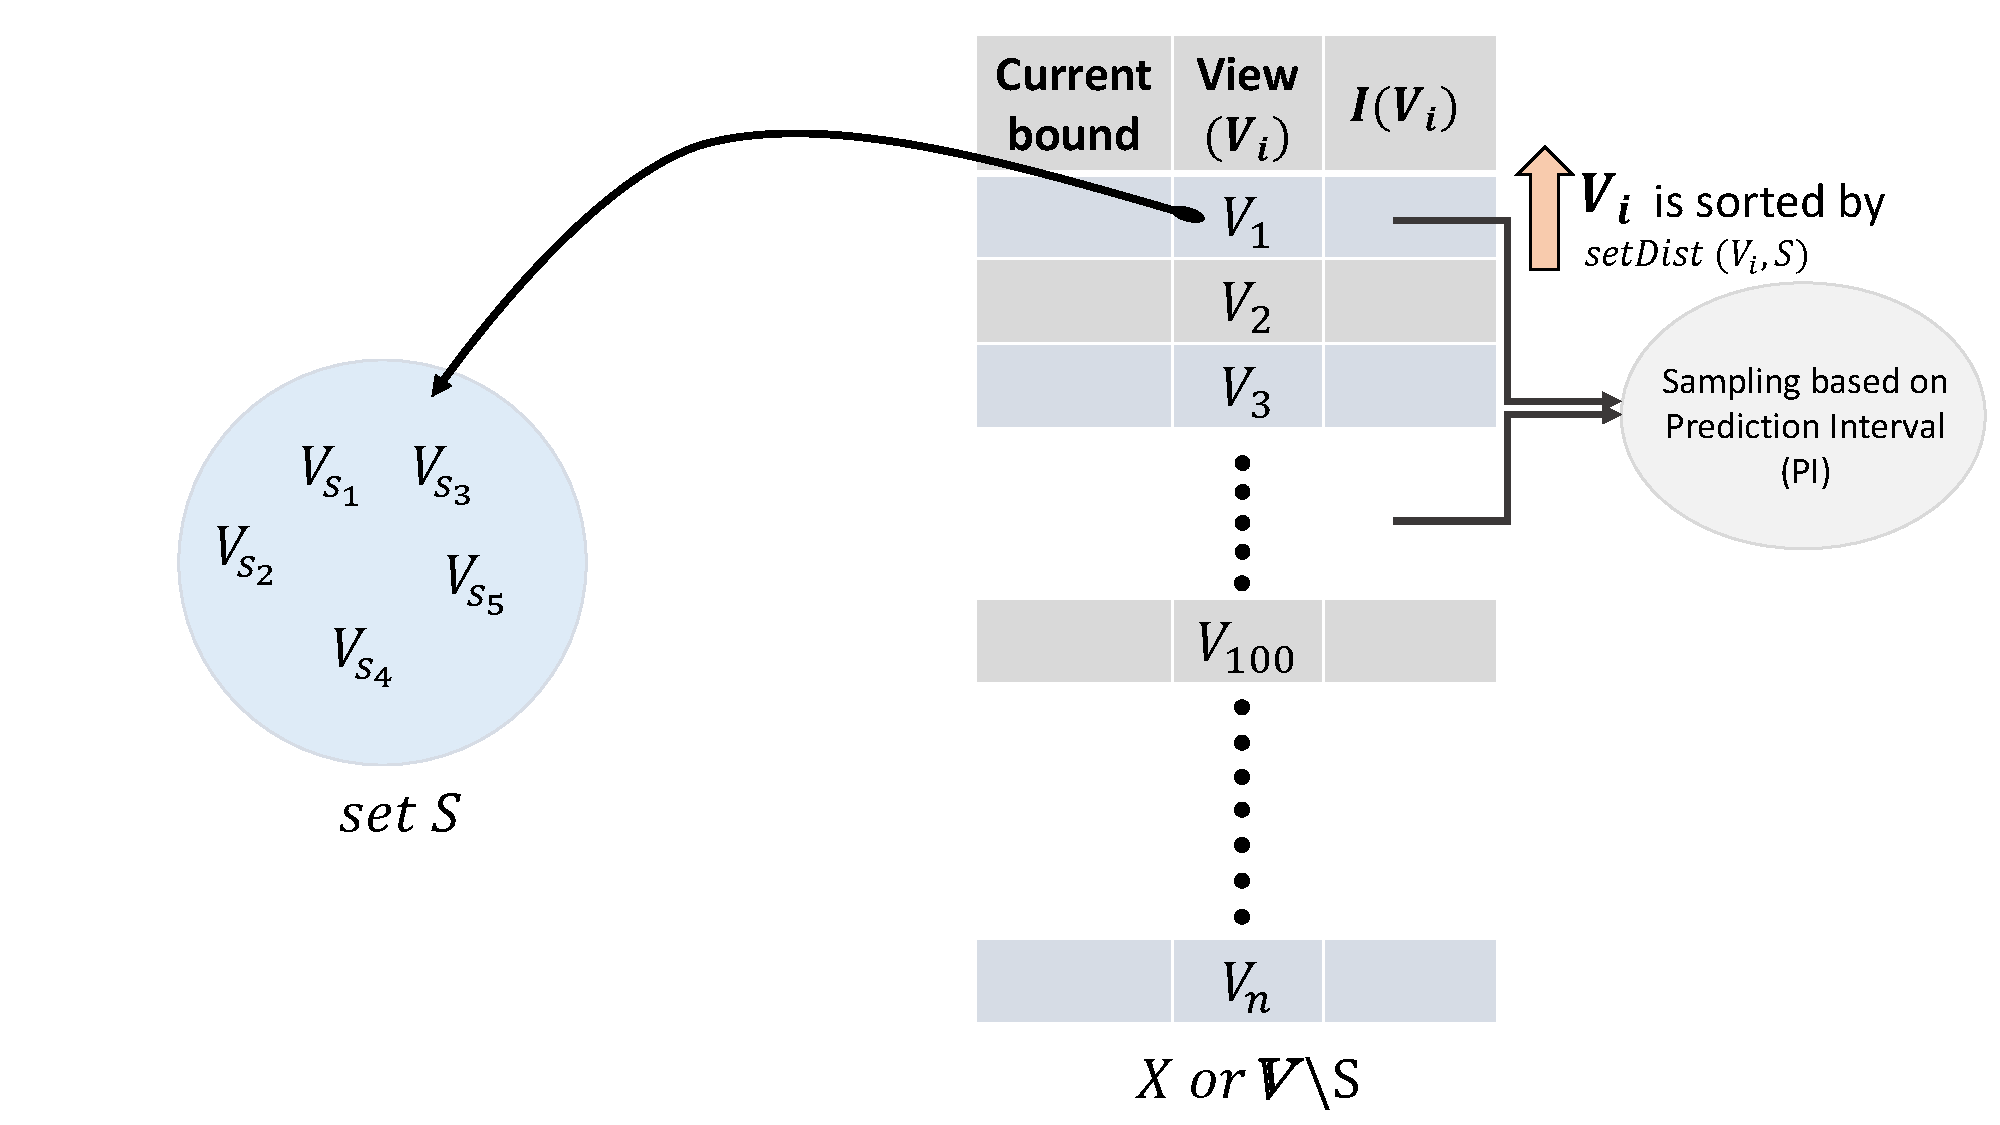
\includegraphics[width=3in]{figures/results/dSwap-Pruning}
%	\caption{dSwap-Pruning: Each candidate view has importance score and $ current bound $. The importance score of view will be generated only for view which its utility score is able to improve set $S$ while using $currentbound$ }
%	\label{fig:dSwap-Pruning}
%\end{figure}

%The idea behind pruning scheme is to minimize the query execution, which is by early prune low quality views. There are two main parameters in pruning scheme: 1) weight of $\lambda$ and 2) the max bound value $I_u$. 

%The weight of $\lambda$ is important due to it determines the contribution of importance score and diversity score. For instance, assume that an analyst wants to get set of views from view recommendation and she uses $\lambda$ = 0.7. The $\lambda$ value equal to 0.7 means that the diversity contribution to the utility score is 70\% and the contribution of importance score will be 30 \%, as it can be seen in equation \ref{objectif_function}. Thus, by setting the $\lambda$ to higher value, the contribution of importance score will be lower and more queries are pruned. This $\lambda$ value is determined by analyst, however, in this experiement 0.5 is used as the default. 